\section{Discussion}

We investigated whether the eye movements used in self-motion perception \cite{clemens2015a} are properly scaled by fixation distance, as required by the geometry. Experiments assessed self-motion perception during either body- and world-centered fixation at two different fixation depths. During far world-centered fixation (where eye movements are small) self-motion was underestimated compared to nearby world-centered fixation (where eye movements are large). Fixation depth did not influence self-motion perception during body-centered fixation (where eye movements are absent). To quantify the relative depth-dependent scaling of eye movements for nearby and far away fixation targets, we fitted a simple linear model to the perceptual and oculomotor responses across four conditions. While two participants show partial scaling, the six remaining participant did not show any sign of scaling.

In addition to the absence of scaling, another explanation is that eye movement information is integrated in a statistically optimal fashion, taking signal noise into account. In the world-fixed condition, this would mean that noisy eye movements in the far fixation are weighed less than those in the less noisy ones in the near fixation condition, giving rise to the observed difference. In this case, similar optimal integration should also occur in the body-fixed fixation condition. As no such differences between the near and far body-fixed fixation conditions have been observed, this is unlikely to be the case.

% FIXME: Change X and Y in paragraph below
As it becomes impossible to distinguish between body- and world-fixed fixation point at far fixation distances, the lack of scaling could - in theory - be explained by participants incorrectly perceiving both the body- and world-fixed far fixation points as being body-fixed. This is unlikely because the target displacement associated with a world-fixed target was between X and Y degrees in our experiment, which is easily perceivable especially given that the target was foveated. This adds confidence to our hypothesis that eye movements indeed influence self-motion perception, with moderate to no scaling for fixation depth.

% Relation to Clemens, 2015
\begin{wrapfigure}{l}[5pt]{0.5\textwidth}
    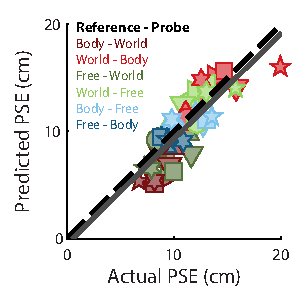
\includegraphics[width=1.0\textwidth]{src/paper4/p4_figure6.pdf}

    \caption{...}
    \label{p4:fig6}
\end{wrapfigure}

In our previous experiment we compared body-fixed to world-fixed fixations at near (50 \si{\centi\metre}) distances only \cite{clemens2015a}. We compared the parameter, $\alpha$, found in that paper with the parameters for the near condition, $\alpha_{50}$, found in the present study. \figref{p4:fig6} shows how well our $\alpha_{50}$ parameter explains the data in our previous paper, the positive correlation between the actual PSEs and those predicted using the model in this paper (stats) adds confidence to the parameter values for  presented here. The average difference between the values found here and those reported previously (see \tabref{p4:tab2}) is 12 \textpm 8 percent-points, indicating a variation of about 12\% on the contribution of the vestibular system versus that of the visual system between the present and our previous paper. While the variation might seem high, keep in mind that the two parameter values presented in this study are fitted on only four conditions, which do not overlap with the two conditions used to fit  parameter  previously.

% Relation to the VOR, e.g. Paige and Busettini
Because the LVOR is commonly thought to keep the eyes stable during linear translation (reference), it also needs to scale with fixation depth. It is therefore possible that both the LVOR and self-motion perception use the same signal. While the fixation point in our experiment causes optokinetically driven eye movements to suplement the LVOR compensation, it is known that the LVOR only partially compensates for the amount of linear translation. If the same signal is also used for self-motion perception, one would expect that, the ratio of the expected LVOR compensation at 50 and 200cm reflect the ones presented in this paper (see \figref{p4:fig5} and \tabref{p4:tab2}).

It has been shown that the relative amount of compensation, or gain, depends on fixation distance angle \cite{paige1989, busettini1994,paige1998}. When fixating far away the gain is closer to 1 compared to fixations closer by. We extrapolated the gains found by Paige, 1989 to the 50 and 200cm fixation distances in our experiment and found gains of 0.50 and 0.68 respectively.

The expected LVOR compensation based on these gains is 5.6 and 3.0 degrees for near and far fixation respectively. The ratio, 1.87, does not match either the 6 participants who do not show any sign of scaling ($\frac{d_{200}}{d_{50}} = 1.07 \pm 0.16$) or the 2 that do ($\frac{d_{200}}{d_{50}} = 3.06 \pm 0.27$), but does match the overall overage of  1.56 \textpm 0.35.

% Conclusion
In summary, fixation depth is not properly taken into account, suggesting that a relatively raw eye movement signal is used in self-motion perception. While efference copies of the eye movement signals or proprioceptive feedback could be directly responsible for the perceived self-motion, it cannot be ruled out that the signals that drive the eye movements, especially those caused by the LVOR, are not causing the reported effect instead.
